\documentclass{ifacconf}
%%%put this lines in ifacconf before hyperref to use it
\makeatletter
\let\old@ssect\@ssect % Store how ifacconf defines \@ssect
\makeatother
\usepackage{amsfonts,amssymb,amsmath,amsthm}

%% set-style letters
\def\AA{{\mathbb{A}}}
\def\BB{{\mathbb{B}}}
\def\CC{{\mathbb{C}}}
\def\DD{{\mathbb{D}}}
\def\EE{{\mathbb{E}}}
\def\FF{{\mathbb{F}}}
\def\GG{{\mathbb{G}}}
\def\HH{{\mathbb{H}}}
\def\II{{\mathbb{I}}}
\def\JJ{{\mathbb{J}}}
\def\KK{{\mathbb{K}}}
\def\LL{{\mathbb{L}}}
\def\MM{{\mathbb{M}}}
\def\NN{{\mathbb{N}}}
\def\OO{{\mathbb{O}}}
\def\PP{{\mathbb{P}}}
\def\QQ{{\mathbb{Q}}}
\def\RR{{\mathbb{R}}}
\def\SS{{\mathbb{S}}}
\def\TT{{\mathbb{T}}}
\def\UU{{\mathbb{U}}}
\def\VV{{\mathbb{V}}}
\def\WW{{\mathbb{W}}}
\def\XX{{\mathbb{X}}}
\def\YY{{\mathbb{Y}}}
\def\ZZ{{\mathbb{Z}}}

%% calligraphic letters
\def\cA{{\mathcal{A}}}
\def\cB{{\mathcal{B}}}
\def\cC{{\mathcal{C}}}
\def\cD{{\mathcal{D}}}
\def\cE{{\mathcal{E}}}
\def\cF{{\mathcal{F}}}
\def\cG{{\mathcal{G}}}
\def\cH{{\mathcal{H}}}
\def\cI{{\mathcal{I}}}
\def\cJ{{\mathcal{J}}}
\def\cK{{\mathcal{K}}}
\def\cL{{\mathcal{L}}}
\def\cM{{\mathcal{M}}}
\def\cN{{\mathcal{N}}}
\def\cO{{\mathcal{O}}}
\def\cP{{\mathcal{P}}}
\def\cQ{{\mathcal{Q}}}
\def\cR{{\mathcal{R}}}
\def\cS{{\mathcal{S}}}
\def\cT{{\mathcal{T}}}
\def\cU{{\mathcal{U}}}
\def\cV{{\mathcal{V}}}
\def\cW{{\mathcal{W}}}
\def\cX{{\mathcal{X}}}
\def\cY{{\mathcal{Y}}}
\def\cZ{{\mathcal{Z}}}
\def\cKL{{\mathcal{KL}}}

%% bold letters
\def\bA{{\bf{A}}}
\def\bB{{\bf{B}}}
\def\bC{{\bf{C}}}
\def\bD{{\bf{D}}}
\def\bE{{\bf{E}}}
\def\bF{{\bf{F}}}
\def\bG{{\bf{G}}}
\def\bH{{\bf{H}}}
\def\bI{{\bf{I}}}
\def\bJ{{\bf{J}}}
\def\bK{{\bf{K}}}
\def\bL{{\bf{L}}}
\def\bM{{\bf{M}}}
\def\bN{{\bf{N}}}
\def\bO{{\bf{O}}}
\def\bP{{\bf{P}}}
\def\bQ{{\bf{Q}}}
\def\bR{{\bf{R}}}
\def\bS{{\bf{S}}}
\def\bT{{\bf{T}}}
\def\bU{{\bf{U}}}
\def\bV{{\bf{V}}}
\def\bW{{\bf{W}}}
\def\bX{{\bf{X}}}
\def\bY{{\bf{Y}}}
\def\bZ{{\bf{Z}}}
\def\ba{{\bf{a}}}
\def\bb{{\bf{b}}}
\def\bc{{\bf{c}}}
\def\bd{{\bf{d}}}
\def\be{{\bf{e}}}
\def\boldf{{\bf{f}}} %different
\def\bg{{\bf{g}}}
\def\bh{{\bf{h}}}
\def\bi{{\bf{i}}}
\def\bj{{\bf{j}}}
\def\bk{{\bf{k}}}
\def\bl{{\bf{l}}}
\def\bm{{\bf{m}}}
\def\bn{{\bf{n}}}
\def\bo{{\bf{o}}}
\def\bp{{\bf{p}}}
\def\bq{{\bf{q}}}
\def\br{{\bf{r}}}
\def\bs{{\bf{s}}}
\def\bt{{\bf{t}}}
\def\bu{{\bf{u}}}
\def\bv{{\bf{v}}}
\def\bw{{\bf{w}}}
\def\bx{{\bf{x}}}
\def\by{{\bf{y}}}
\def\bz{{\bf{z}}}

%% other symbols
\DeclareMathOperator{\1}{\mathbf{1}}
\DeclareMathOperator{\0}{\mathbf{0}}
\DeclareMathOperator{\Id}{I}
\newcommand{\td}{\mathfrak{t}} % discrete-time 
\newcommand{\tr}{^\top}

%% operators
\DeclareMathOperator{\col}{col}
\DeclareMathOperator{\diag}{diag}
\DeclareMathOperator{\blkdiag}{blkdiag}
\DeclareMathOperator{\rank}{rank}
\DeclareMathOperator{\dis}{d}
\DeclareMathOperator{\sat}{sat} 
\DeclareMathOperator{\convhull}{\textbf{co}}
\DeclareMathOperator{\argmin}{argmin}
\DeclareMathOperator{\argmax}{argmax}
\DeclareMathOperator{\spec}{spec}
\def\He#1{\texttt{\rm{He}}\left\{{#1}\right\}}
\DeclareMathOperator{\trace}{tr}
\newcommand{\Imag}{\mathrm{Im}}

%% shortcuts
\newcommand{\norm}[1]{\lvert #1\rvert}
\newcommand{\wnorm}[2]{\lvert #1\rvert^2_{#2}}
\newcommand{\pderiv}[2]{\dfrac{\partial #1}{\partial #2}}
\newcommand{\pdef}[1]{\SS_{\succ0}^{#1}}
\newcommand\psemidef[1]{\SS_{\succeq0}^{#1}}
\newcommand{\bmx}[1]{\left[\begin{matrix}#1\end{matrix}\right]}
\newcommand{\pmx}[1]{\left(\begin{matrix}#1\end{matrix}\right)}
\newcommand{\smallpmat}[1]{\left(\begin{smallmatrix} #1 \end{smallmatrix} \right)}
\newcommand{\smallqmat}[1]{\left[\begin{smallmatrix} #1 \end{smallmatrix} \right]}
\newcommand{\overbar}[1]{\mkern 1.5mu\overline{\mkern-1.5mu#1\mkern-1.5mu}\mkern 1.5mu}
\renewcommand{\underbar}[1]{\mkern 1mu\underline{\mkern-1mu#1\mkern-1mu}\mkern 1mu}

\usepackage{hyperref}
\usepackage{graphicx}
\usepackage{float}

% SCRIPTS FOR DOUBLE AND SINGLE IMAGE

% \begin{figure}[H]
%     \centering
%     \begin{subfigure}{0.4\textwidth}
%     \includegraphics[width=\textwidth]{}
%     \caption{}
%     \label{}
%     \end{subfigure}
%     \hfill
%     \begin{subfigure}{0.55\textwidth}
%     \includegraphics[width=\textwidth]{}
%     \caption{}
%     \label{}
%     \end{subfigure}
%     \caption{}
%     \label{}
% \end{figure}

% \begin{figure}[H]
%     \centering
%     \includegraphics[width=0.65\textwidth]{}
%     \caption{}
%     \label{}
% \end{figure}

\usepackage{natbib}
%\usepackage{booktabs}
%%%put this lines in ifacconf after hyperref to use it
\makeatletter
\def\@ssect#1#2#3#4#5#6{%
  \NR@gettitle{#6}% Insert key \nameref title grab
  \old@ssect{#1}{#2}{#3}{#4}{#5}{#6}% Restore ifacconf's \@ssect
}
\makeatother

%%theorems
\theoremstyle{plain}
\newtheorem{theorem}{Theorem}
\newtheorem{proposition}{Proposition}
\newtheorem{assumption}{Assumption}
\newtheorem{lemma}{Lemma}
\newtheorem{remark}{Remark}
\newtheorem{definition}{Definition}
\newtheorem{corollary}{Corollary}
\newtheorem{problem}{Problem}
\newenvironment{proof}{\paragraph*{Proof:}}{\hfill$\square$}

\begin{document}
\begin{frontmatter}

\title{Draft of paper}

\author[First]{Marco Sterlini}
\author[Second]{Samuele Zoboli}
\author[Second]{Sophie Tarbouriech}

\address[First]{University di Trento, Trento, Italy (e-mail: marco.sterlini@studenti.unitn.it) }
\address[Second]{LAAS-CNRS, Université de Toulouse, CNRS, Toulouse, France (e-mail:bu) }


\begin{abstract}
\textbf{INSERT ABSTRACT}
\end{abstract}

\begin{keyword}
\textbf{INSERT KEYWORDS}
\end{keyword}

\end{frontmatter}

\section{Introduction}
\textbf{INSERT INTRODUCTION}\\
\emph{Notation:} $\NN, \RR^{n}, \RR^{n \times m}$ denote the set of natural non-negative integers, the set of real vectors of dimension $n$ and the set of real matrices of dimension $n \times m$, respectively. For any matrix $A$, $A\tr$ is its transpose. For any square matrix $A$, the operator $\He{ A } = A + A\tr$ is defined. $\texttt{diag}(A_1, A_2)$ is a block-diagonal matrix with block-diagonal matrices $A_1$ and $A_2$. For a partitioned matrix, the symbol $\star$ stands for symmetric blocks. $\1_n = \bmx{1 & \dots & 1}\tr \in \NN^{n \times 1}$. We identify with subscript $i$ the $i$-th element of a vector or the $i$-th row of a matrix.

\section{Problem Formulation}
We consider the non-linear discrete-time system stabilized by a Neural Network (NN) controller represented in figure \ref{fig:first_scheme} described by:
\begin{equation}
  x^{+} = A x + B \texttt{sat}(\bar{u}) + C \Phi(E x) + D d 
\end{equation}
where the saturation function \texttt{sat} is defined as:
$$
    \texttt{sat}(\bar{u}) = \texttt{sign}(\bar{u})\text{min}(|\bar{u}|, \hat{u})
$$
with $\hat{u}$ the limit of the input signal, $x \in \RR^{n_x}$ the state vector, $\bar{u} \in \RR^{n_u}$ the raw output of the controller, $d \in \RR^{n_d}$ a constant disturbance input  and $\Phi \in \RR^{n_q}$ the representation of the non-linearity of the system. 
\begin{assumption}\label{ass:nonlin}
We assume that $\Phi$ satisfies some local quadratic abstraction for some $\underline{\mu}, \bar{\mu} > 0 \in \RR^{n_q}, \bar{S}, \bar{Q}, \bar{W} \in \RR^{n_q \times n_q}$
\begin{equation}\label{eqn:nonlin-set}
\forall v \in \bar{S} = \left\{ v \in  \RR^{n_q} : - \underline{\mu}_i \leq v_i \leq \bar{\mu}_i, i \in \pmx{1 & \dots & n_q} \right\} 
\end{equation}
\begin{equation}\label{eqn:nonlin-inclusion}
\bmx{x \\ \Phi(x)}\tr \bmx{\bar{S} & \bar{Q} \\ \star & \bar{W}} \bmx{x \\ \Phi(x)} \geq 0
\end{equation}
\end{assumption}\textcolor{red}{Please help in adding details about $\Phi$ since it's NOLCOS}.

\begin{figure}[H]
    \centering
    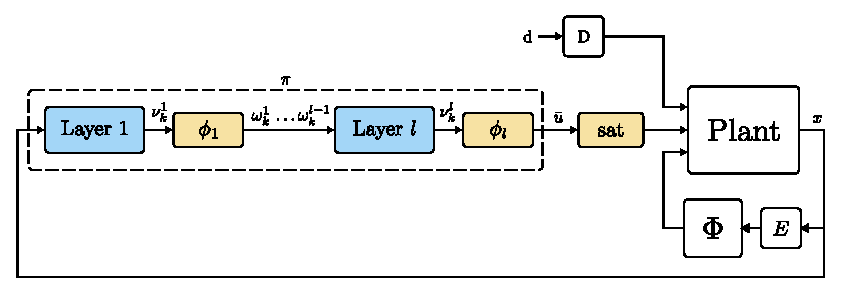
\includegraphics[width=0.45\textwidth]{Figures/first_scheme}
    \caption{Feedback system}
    \label{fig:first_scheme}
\end{figure}

The controller is implemented as a Multi Layer Perceptron (MLP) with $l$ layers, each with $n_{\phi_i}, i \in \left\{ 1, \dots, l\right\}$ neurons, all activation functions are saturation functions, represented by $\phi_i$. The objective is to design an Event-Triggering Mechanism (ETM) that allows to ease the computational burden associated with the computation of many non-linear activation functions providing at the same time sufficient sector conditions to handle the non-linearity of the system and the controller. The controller $\pi$ is defined by:
\begin{equation}\label{eqn:nn-equations}
  \begin{aligned}
  \hat{\omega}^{0}(k) &= x(k) \\
  \nu^{i}(k) &= W^{i} \hat{\omega}^{i - 1}(k) + b^{i}, i \in \left\{ 1, \dots, l \right\}\\
  \omega^{i}(k) &= \phi_i(\nu^i(k))\\
  \bar{u}(k) &= \phi_l(\nu^l(k))
  \end{aligned} 
\end{equation}
with $\nu^i(k) \in \RR^{n_{\phi_i}}$ the input to the $i$-th activation function $\phi^i: \RR^{n_{\phi_i}} \to \RR^{n_{\phi_i}}$, $\omega^i(k), \hat{\omega}^i(k) \in \RR^{n_{\phi_i}}$ the current and last forwarded output respectively. The weights $W^i \in \RR^{n_{\phi_i} \times n_{\phi_{i-1}}}$ and biases $b^i \in \RR^{n_{\phi_i}}$ define the affine operation of each layer. The saturation function application is to be intended element-wise and will be denoted as $\phi^i(\nu^i(k)) = \left[ \varphi(\nu^i_1(k)), \dots, \varphi(\nu^i_{n_{\phi_i}}(k)) \right]$ and $\varphi: \RR \to \RR$ is the scalar activation function assumed to be symmetric and identical for every neuron. Adopting the same notation as in \cite{css-paper} we define the controller policy in a condensed form. Denoting the augmented vectors:
\begin{equation*}
  \nu = \bmx{\nu^1 \\ \vdots \\ \nu^l}, \omega = \bmx{\omega^1 \\ \vdots \\ \omega^l}, \phi = \bmx{\phi^1(\nu^1) \\ \vdots \\ \phi^l(\nu^l)} 
\end{equation*}
with $n_{\phi} = \sum_{i=1}^{l} n_{\phi_i}$ and $\phi: \RR^{n_{\phi}} \to \RR^{n_{\phi}}$ the combined non-linearity we have $\omega = \phi(\nu)$. Finally, conditions \eqref{eqn:nn-equations} can be rewritten as:
\begin{equation*}
  \bmx{u(k)\\ \nu(k)} = \overbar N \bmx{x(k) \\ \omega(k) \\ 1} 
\end{equation*}
where
\begin{equation}\label{eqn:first-N}
  \overbar N = \bmx{
    \begin{array}{c | c c c c | c}
      \0 & \0 & \dots & \0 & W^l & b^l \\ 
      \hline
      W^1 & \0 & \dots & \0 & \0 & b^1 \\
      \0 & W^2 & \dots & \0 & \0 & b^2 \\
      \vdots & \vdots & \ddots & \vdots & \vdots & \vdots \\
      \0 & \0 & \dots & W^{l-1} & \0 & b^{l-1}
    \end{array}
  }
\end{equation}
Similarly as in \cite{css-extended} we implement an ETM in every layer of the controller, we add also a final one to the output that will be used to further reduce the total number of events and calls to the non-linear functions. The system and the controller are now described by figure \ref{fig:second_scheme}.
\begin{figure}[H]
    \centering
    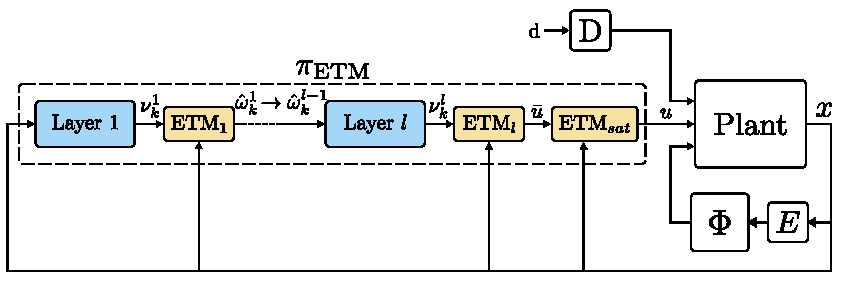
\includegraphics[width=0.45\textwidth]{Figures/second_scheme}
    \centering
    \caption{Feedback system subject to ETM in the controller}
    \label{fig:second_scheme}
\end{figure}
The dynamics will be rewritten as:
\begin{equation}\label{eqn:system-dynamics}
  x^{+} = A x + B u + C \Phi(E x) + D d
\end{equation}
with $u \in \RR^{n_u}$ the output of the controller subject to the ETM. This modification required to redefine the matrix $N$ defined in the controller policy \eqref{eqn:first-N} as:
\begin{equation}\label{eqn:last-N}
  N = \bmx{
    \begin{array}{c | c c c c | c}
      \0 & \0 & \dots & \0 & \Id & 0 \\ 
      \hline
      W^1 & \0 & \dots & \0 & \0 & b^1 \\
      \0 & W^2 & \dots & \0 & \0 & b^2 \\
      \vdots & \vdots & \ddots & \vdots & \vdots & \vdots \\
      \0 & \0 & \dots & W^l & \0 & b^l
    \end{array}
  } = \bmx{
    \begin{array}{c | c | c}
    N_{u x} & N_{u \omega} & N_{u b} \\
    \hline
    N_{\nu x} & N_{\nu \omega} & N_{\nu b}
    \end{array} 
  }
\end{equation}


The system is compliant with the assumptions of \citep[Lemma 2]{css-extended} that allow us to define the following expressions regarding the equilibrium points $\left( x_*, u_*, \nu_*, \omega_* \right)$ of the system and controller given $x_*$, defining the matrices:
\begin{equation}
    \begin{aligned}
         &R = (\Id - N_{\nu \omega})^{-1}\\
         &R_{\omega} = N_{u x} + N_{u \omega} R N_{\nu x}\\
         &R_b = N_{u \omega} R N_{\nu b} + N_{u b}
    \end{aligned}
\end{equation}

With $R$ always invertible due to $N_{\nu \omega}$ always invertible due to its lower triangular structure. We find the equilibrium of the state by the use of a numerical solver that minimizes the following expression since it is no longer explicit due to the non-linearity $\Phi$. Given a constant disturbance $\bar{d}$:
\begin{equation}
  x_* = \min_{x} \left[(A + B R_{\omega} - \Id) x + C \Phi(E x) + D \bar{d} + B R_b \right]
\end{equation}
\begin{equation}\label{eqn:equilibrium}
  \bmx{u_* \\ \nu_*} = N \bmx{x_* \\ \omega_* \\ 1}; \ \  
  \begin{aligned}
    \omega_* &= \nu_*\\
    \nu_* &= R N_{\nu x} x_* + R N_{\nu b}\\
    u_* &= R_{\omega} x_* + R_b
  \end{aligned}
\end{equation}
All the non-linearity of the system and the controller are selected as saturation functions. With respect to \citep[Lemma 3]{css-extended}, we declare the local sector conditions that hold for every state included in the following set:

\begin{remark}\label{rem:sec-set}
\emph{For $i \in \left\{ 1, \dots, l \right\}$ given a matrix $G^i \in \RR^{n_{\phi_i} \times n_x}$, if $x$ belongs to the set}
\begin{equation}\label{eqn:inclusion-set}
S = \left\{ x \in \RR^{n_x} : -\bar{\nu}^i - \bar{\nu}^i_* \leq G^i (x - x_*) \leq \bar{\nu}^i - \nu_*^i \right\} 
\end{equation}

\emph{Then the following quadratic constraint holds for any diagonal positive definite matrix $T^i \in \RR^{n_{\phi_i} \times n_{\phi_i}}$:}
\begin{equation}\label{eqn:first_sec_cond}
  \left[ \nu^i - \omega^i \right]\tr T^i \left[ G^i (x - x_*) - (\omega^i - \omega^i_*) \right] \leq 0
\end{equation}\end{remark}
Where $\bar{\nu}^i$ is the saturation level of the $i$-th layer.

In order to have a lighter notation the dead-zone vector  will be defined as $\psi^i = \nu^i - \omega^i$ and $\hat{\psi}^i = \nu^i - \hat{\omega}^i$. Furthermore, all following discussions will take into account incremental variables with respect to their equilibrium, denoted with a tilde, i.e. $\tilde{x} = x - x_*$. Considering \eqref{eqn:equilibrium} we have $\psi_* = \nu_* - \omega_* = 0$ hence $\tilde{\psi} = \psi$. We define $\xi^i = \bmx{\tilde{x}\tr & \tilde{\psi}_i\tr & \tilde{\nu}_i\tr}\tr$ and $\hat{\xi}^i = \bmx{\tilde{x}\tr & \hat{\tilde{\psi}}_i\tr & \tilde{\nu}_i\tr}\tr$, then the overall sector conditions \eqref{eqn:first_sec_cond} can be rewritten with no loss of generality $\forall i \in \pmx{1 & \dots & l}$ as:
\begin{equation}\label{eqn:sec_cond}
\begin{aligned}
    &({\tilde{\psi}^i})\tr T^i \bmx{G^i \tilde{x} + \tilde{\psi}^i - \tilde{\nu}^i} = {\xi^i}\tr \bmx{0 & 0 & 0\\
    T^i G^i & T^1 & -T^1\\
    0 & 0 & 0} \xi^i = \\
    &= {\xi^i}\tr \Omega^i \xi^i \leq 0
\end{aligned}
\end{equation}

\begin{remark}\label{rem:sec-cond}
Note how ensuring ${\xi^i}\tr \Omega^i \xi^i < 0$ guarantees that the sector condition \eqref{eqn:sec_cond} holds.
\end{remark}

We can express now the new interdependency between the variables of interest:
\begin{equation}\label{eqn:incremental}
  \begin{aligned}
    \tilde{u} &= R_{\omega} \tilde{x} - N_{u \omega} R \tilde{\psi}\\
    \tilde{\nu} &= R N_{\nu x} \tilde{x} + (\Id - R) \tilde{\psi}
  \end{aligned}
\end{equation}

\section{Main Results}

Taking inspiration from \citep[Proposition 1, Lemma 3]{css-extended} we design the ETM for the output of each layer of the controller and the final output.

\subsection{Event-triggering mechanism}
An ETM works by triggering an event that will update the current layer and propagate its value across the network. 
In the precedent work \cite{css-extended} the triggering function is defined on the basis of the saturation sector conditions in the form \eqref{eqn:sec_cond}. The ETM was defined as:
\begin{equation}
  \hat{\omega}^{i}(k) = \begin{cases}
    \phi^i(\nu^i(k)) & \text{if } {\hat{\xi^i}}\tr \Omega^i \hat{\xi^i} > 0\\
    \hat{\omega}^{i}(k-1) & \text{otherwise}
  \end{cases}
\end{equation}

This approach acts as a static ETM triggering an event immediately after the sector conditions are violated. Inspired by the work of \cite{data-driven} we define a dynamic quantity to be implemented in the ETM triggering condition. The idea is to lower the conservatism of the controller by introducing a time-varying threshold that will adapt to the current state of the system and controller reducing the overall number of events and computational burden. The new triggering function for the new \emph{dynamic-ETM} for the $i$-th layer is defined as:
\begin{equation}\label{eqn:dynamic_trig}
  \hat{\omega}^{i}(k) = \begin{cases}
    \phi^i(\nu^i(k)) & \text{if } {\hat{\xi^i}}\tr \Omega^i \hat{\xi^i} > \rho^i \eta_i\\
    \hat{\omega}^{i}(k-1) & \text{otherwise}
  \end{cases};
\end{equation}

Where $\eta^i$ characterized by the following dynamics:
\begin{equation}\label{eqn:eta_dynamics}
  {\eta^i}^+ = \rho^i \eta^i - {\hat{\xi^i}}\tr \Omega^i \hat{\xi^i}\quad  \forall i \in \left( 1, \dots, l \right) 
\end{equation}

We denote a condensed notation by taking into account all conditions for each layer
\begin{equation}
\begin{aligned}
   \bR &= \text{diag} \pmx{\rho^1 & \dots & \rho^l }\\
   \mathbf{\Psi} &= \bmx{ {\hat{\xi^1}}\tr \Omega^1 \hat{\xi^1} & \dots & {\hat{\xi^l}}\tr \Omega^l \hat{\xi^l}}\tr\\
   \boldsymbol{\eta} &= \bmx{ \eta^1 & \dots & \eta^l}\tr   
\end{aligned}
\end{equation}

The ETM triggering condition and dynamic thresholds' dynamics can be rewritten in an element-wise fashion as:
\begin{equation}
\begin{aligned}
    \boldsymbol{\eta}^+ &= \bR \boldsymbol{\eta} - \mathbf{\Psi}\\
    \mathbf{\Psi} &> \bR \boldsymbol{\eta}
\end{aligned}
\end{equation}

\subsection{Finsler Lemma application}
After the implementation of the dynamic threshold a further improvement of the triggering condition has been taken in consideration. By recalling the triggering condition:
$$
\hat{{\xi^i}}\tr \Omega^i \hat{\xi^i} > \rho^i \eta^i
$$
Intuitively the lower the left-hand term of the inequality the lower will be the number of triggered events. Unfortunately $\Omega^i$ structure is non-flexible due to his strict relation with the sector condition expression. The following lemma addresses the issue by designing some triggering matrices that guarantee a lower update rate for each layer by the use of Finsler's lemma:

\begin{lemma}\label{lem:finsler} \emph{Considering the triggering policy \eqref{eqn:dynamic_trig}, $R^i$ such that ${\xi^i}\tr = \!R^i \bmx{\tilde{x} & \tilde{\psi} & \tilde{\nu}}\tr\! = R^i \xi\tr$, with reference to the structure in \eqref{eqn:sec_cond} and assuming \eqref{eqn:incremental} holds for some $\underline{\xi}, \bar{\xi} \in \RR^{n_x + 2n_{\phi}}$ such that $\forall \xi \in \left[ \underline{\xi}, \bar{\xi}\right]$, if $\exists X^i \in\! \RR^{(nx + 2n_{\phi_i}) \times (nx + 2n_{\phi_i})},$ $N^i_1 \in \RR^{n_x \times n_{\phi_i}}, N^i_2, N^i_3 \in \RR^{n_{\phi_i} \times n_{\phi_i}}$ a diagonal matrix $T^i > 0 \in \RR^{n_{\phi_i} \times n_{\phi_i}}, G^i \in \RR^{n_{\phi_i} \times n_x}$ such that:
\begin{equation}\label{eqn:finsler}
     {R^i}\tr\! He\left\{X^i - \Omega^i\right\}\! R^i + He\left\{ \smallpmat{N^i_1\\ N^i_2\\ N^i_3}\! \pmx{R N_{\nu x} & \Id - R & -\Id}\right\} \leq 0
\end{equation}
Then we have ${\xi^i}\tr X^i \xi^i \leq {\xi^i}\tr \Omega^i \xi^i$}
\end{lemma}

\begin{proof} By pre and post multiplying for $\xi$ the previous expression we end up with
$$
    {\xi^i}\tr\! He \!\left\{\!X^i \!-\! \Omega^i\right\} \xi^i + He\!\left\{ \xi\tr\! \smallpmat{N^i_1\\ N^i_2\\ N^i_3}\! \smallpmat{R N_{\nu x} & \Id - R & -\Id} \xi\! \right\}\! \leq 0
$$
By expanding the term $\pmx{R N_{\nu x} & \Id - R & -\Id} \xi$ we end up with condition \eqref{eqn:incremental} meaning that the expression is reduced to
$$
    {\xi^i}\tr \He{X^i - \Omega^i} \xi^i \leq 0
$$
By further expanding the expression and considering that it is eventually reduced to a scalar for which it holds that the transpose is equivalent to itself we obtain:  
\begin{equation*}
\begin{aligned}
    &{\xi^i}\tr (X^i + {X^i}\tr) \xi^i \leq {\xi^i}\tr (\Omega^i + {\Omega^i}\tr) \xi^i\\
    &2 {\xi^i}\tr X^i\xi^ \leq 2 {\xi^i}\tr \Omega^i \xi^i\\
    & {\xi^i}\tr X^i \xi^i \leq {\xi^i}\tr \Omega^i \xi^i
\end{aligned}
\end{equation*}
\end{proof}

Assuming we have the $X^i$ matrices $i \in \left\{1, \dots, l \right\}$ we rewrite the triggering conditions for each layer:
\begin{equation}\label{eqn:etm-trigger}
  \hat{\omega}^{i}(k) = \begin{cases}
    \phi^i(\nu^i(k)) & \text{if } {\xi^i}\tr X^i \xi > \rho^i \eta^i(k)\\
    \hat{\omega}^{i}(k-1) & \text{otherwise}
  \end{cases}
\end{equation}
\begin{remark}\label{rem:eta-positive} \emph{Similarly as in \citep[Lemma 3]{data-driven} it is possible to demonstrate how $\eta^i$ being the dynamic threshold of layer $i$ is always non-negative for any $\rho^i \in [0, 1)$, $\eta^i_0 \geq\ 0$} \end{remark}
With respect to \eqref{eqn:etm-trigger} and \eqref{eqn:eta_dynamics} we have two possible occurrences:
\begin{itemize}
    \item $\hat{{\xi^i}}\tr X^i \hat{\xi^i} \leq \rho^i \eta^i$: it's trivial to verify that ${\eta^i}^+ = \rho^i \eta^i - \hat{{\xi^i}}\tr X^i \hat{\xi^i} \geq 0 $
    \item $\hat{\xi^i}\tr X^i \hat{\xi^i} > \rho^i \eta^i$: in this case an event is triggered and the vector $\hat{\xi^i}$ gets updated to $\xi^i$ after the activation function application, in this situation \eqref{eqn:sec_cond} is met and with respect to remark \ref{rem:sec-cond} and Lemma \ref{lem:finsler} we have ${\xi^i}\tr X^i \xi^i < {\xi^i}\tr \Omega^i \xi^i < 0$. Once again we have ${\eta^i}^+ = \rho^i \eta^i - {\xi^i}\tr X^i \xi^i > 0 $
\end{itemize}
By denoting $\bX = \text{diag} \pmx{R_1\tr X^1 R_1 & \dots & R_l\tr X^l & R_l} $ and $\xi = \bmx{\tilde{x} & \tilde{\psi} & \tilde{\nu}}\tr$
$$
\mathbf{\Psi_x} = \pmx{\Id_l \otimes \xi}\tr\! \bX \pmx{\1_l \otimes \xi}
$$
the ETM triggering condition and dynamic thresholds' dynamics can be rewritten in an element-wise fashion as:
\begin{equation}
\begin{aligned}
    \boldsymbol{\eta}^+ &= \bR \boldsymbol{\eta} - \mathbf{\Psi_x}\\
    \mathbf{\Psi_x} &> \bR \boldsymbol{\eta}\end{aligned}
\end{equation}

\subsection{Lyapunov conditions}
In this section we will provide sufficient conditions for the stability of the system and the controller under the form of Linear Matrix Inequalities (LMIs) with the guarantee of local asymptotic stability. The solution of the problem will also provide the matrices $X^i$ and the parameters $\rho^i$ that will be used in the ETM triggering conditions along with an estimate of the Region Of Attraction (ROA) of the equilibrium point. 

We will first introduce a more compact notation for the system dynamics as long as some auxiliary matrices:
\begin{equation}\label{eqn:auxiliary}
\begin{aligned}
    \bar{A} &= A + B R_{\omega}\\
    \bar{B} &= -B N_{u \omega} R\\
    \tilde{x}^+ &= \bar{A}\tilde{x} + \bar{B}\tilde{\psi} + C \tilde{\Phi}\\
R_{\nu} &= \bmx{
  \Id & 0 & 0 \\
  0 & \Id & 0 \\
  R N_{\nu x} & \Id - R & 0\\
} \in \RR^{(n_x + n_{\phi} + n_q) \times (n_x + 2 n_{\phi})}\\
R_s &\in \RR^{(n_x + n_{\phi} + n_q) \times (n_x + n_q)}
\end{aligned}
\end{equation}

\begin{figure*}
\begin{subequations}\label{eqn:LMI}
\begin{align}\label{eqn:lyapunov}
  &\Xi =\bmx{
  \begin{array}{c|c}
  \bmx{\bar{A}\tr\\
  \bar{B}\tr\\
  C\tr
  } P \bmx{\bar{A} & \bar{B} & C} - \bmx{
  P & 0 & 0\\
  0 & 0 & 0\\
  0 & 0 & 0
  } - (\1_l \otimes R_{\nu})\tr \He{\bX} (\1_l \otimes R_{\nu})
   + R_s\tr \bmx{
    S & Q\\
    \star & W
  }  R_s\hspace{.1em}& 0\\[1.5em]
\hline \\[-0.9em]
  0 & \hspace{.1em} 2 (\bR - \Id)
  \end{array}} < 0\\
  &\bmx{
    P & {Z_j^i}\tr\\
    \star & 2 \alpha T^i_{j,j} - \alpha^2 (\hat{\nu}_j^i)^{-2}
  } \geq 0 \qquad \forall i \in \left\{ 1, \dots, l \right\}, j \in \left\{ 1, \dots, n_{\phi_i} \right\} \label{eqn:inclusion}\\
  &{R^i}\tr\! \He{X^i - \Omega^i} R^i + He\left\{ \pmx{N^i_1\\ N^i_2\\ N^i_3} \pmx{R N_{\nu x} & \Id - R & -\Id}\right\} \leq 0 \qquad \forall i \in \left\{ 1, \dots, l \right\} \label{eqn:finsler_constraint}\\
  &\bmx{P & {E_i}\tr \\ \star & \hat{\mu_i}^2} \geq 0 \qquad \forall i \in \left\{1, \dots, n_q \right\} \label{eqn:nonlin-inclusion-constraint}
\end{align}
\end{subequations}
\vspace{.5em}
\hrule
\end{figure*}
% \begin{figure*}
% \begin{equation}\label{eqn:first-step}
%  \bmx{\tilde{x} \\ \tilde{\psi} \\ \tilde{\Phi}}\tr \left( \!
%   \bmx{\bar{A}\tr\\
%   \bar{B}\tr\\
%   C\tr
%   } P \bmx{\bar{A} & \bar{B} & C} - \bmx{
%   P & 0 & 0\\
%   0 & 0 & 0\\
%   0 & 0 & 0
%   } \right) \bmx{\tilde{x} \\ \tilde{\psi} \\ \tilde{\Phi}}
%  - \pmx{\1_l \otimes \xi}\tr \He{\bX} \pmx{\1_l \otimes \xi}
%  + \bmx{\tilde{x}\\ \tilde{\Phi}}\tr\! \bmx{S & Q\\ \star & W} \bmx{\tilde{x} \\ \tilde{\Phi}}
%  + \sqrt{\boldsymbol{\eta}}\tr \He{\bR - \Id} \sqrt{\boldsymbol{\eta}}
% \end{equation}
% \vspace{.5em}
% \hrule
% \end{figure*}

\begin{theorem}\label{thm:stability} \emph{ Consider the control system in \eqref{eqn:system-dynamics} and the controller $\pi_{\text{ETM}}$ in \eqref{eqn:nn-equations}. Assuming the existence of the matrices $P = P\tr > 0 \in \RR^{n_x \times n_x}$,} $T = \text{diag} \pmx{T^1 & \dots & T^l} \in \RR^{n_{\phi} \times n_{\phi}} > 0$, \emph{$Z = \smallpmat{{Z^1}\tr & \dots & {Z^l}\tr}\tr \in \RR^{n_{\phi} \times n_x}$, $\bR > 0$, $\bX$, $N^i_1, N^i_2, N^i_3 \ \forall i \in \left\{ 1, \dots, l \right\}$, $S \in \RR^{n_x \times n_x}, Q \in \RR^{n_x \times n_q}, W \in \RR^{n_q \times n_q}$ and a scalar $\alpha > 0$ such that the matrix inequalities \eqref{eqn:lyapunov}, \eqref{eqn:inclusion}, \eqref{eqn:finsler} hold, where $\hat{\nu}_j^i = \min(|-\bar{\nu}_j^i - \nu^i_{*, j}|,|\bar{\nu}_j^i - \nu^i_{*, j}|)$, $
\hat{\mu}_i = \min(|-\underline{\mu}_i - v_i^*|,|\bar{\mu}_i - v_i^*|)$ and $G^i = (T^i)^{-1} Z^i\ \forall i \in \left\{1, \dots, l \right\}$
Then the point $(x, \boldsymbol{\eta}) = (x_*, \0)$ is Locally Exponentially Stable (LES) with a ROA that includes the ellipsoid $\cE(P, x_*) = \left\{ x \in \RR^{n_x}, \boldsymbol{\eta} \in \RR^{l} : \tilde{x}\tr P \tilde{x} + \He{\1_l\tr \boldsymbol{\eta}} \leq 1\right\}$}
\end{theorem}


\begin{proof}
By exploiting the inequality $$\bmx{\alpha (\hat{\nu}^i_j)^{-2} - T^i_{j, j}}(\hat{\nu}^i_j)^2\bmx{\alpha (\hat{\nu}^i_j)^{-2} - T^i_{j, j}} \geq 0$$ having $(T^i_{j,j})^2(\hat{\nu}^i_j)^2 \geq 2 \alpha T^i_{j,j} - \alpha^2 (\hat{\nu}_j^i)^{-2}$ and assuming \eqref{eqn:inclusion} we state:
$$
\bmx{
P & (T^i_{j,j} G^i_j)\tr\\
\star & (T^i_{j,j})^2(\hat{\nu}^i_j)^2
} \geq 
\bmx{
P & {Z_j^i}\tr\\
\star & 2 \alpha T^i_{j,j} - \alpha^2 (\hat{\nu}_j^i)^{-2}
} \geq 0
$$
That implies
$$
\bmx{
P & 0 & (T^i_{j,j} G^i_j)\tr\\
0 & 2 \Id & 0\\
\star & 0 &(T^i_{j,j})^2(\hat{\nu}^i_j)^2
} \geq 0
$$
We initially assume the positivity of $\boldsymbol{\eta}$, by pre and post multiplying for $\bmx{\tilde{x}\tr, \sqrt{\boldsymbol{\eta}}, 1}\tr$ and its transpose and applying Schur's complement we obtain
$$
\bmx{\tilde{x}\\ \sqrt{\boldsymbol{\eta}}}\tr \bmx{P & 0\\ 0 & 2 \Id} \bmx{\tilde{x}\\ \sqrt{\boldsymbol{\eta}}} \geq \tilde{x}\tr \frac{(G^i_j)\tr (G^i_j)}{\hat{\nu^i_j}^2} \tilde{x}
$$
This ensures $\cE(P, x_*) \subseteq S$ defined in Remark \ref{rem:sec-set}. Now assuming \eqref{eqn:finsler_constraint} hold $\forall (x, \boldsymbol{\eta}) \in \cE(P, x_*)$, by the application of Lemma \ref{lem:finsler} we ensure $\boldsymbol{\eta} > 0$ through Remark \ref{rem:eta-positive}. Considering \eqref{eqn:nonlin-inclusion-constraint} we have
$$
\bmx{P & 0 & E_i\tr \\
0 & 2 \Id & 0 \\
E_i & 0 & \hat{\mu_i}^2} \geq 0
$$
By expressing $v_i = E_i x$ and pre and post multiplying by $\bmx{\tilde{x}\tr & \tilde{\Phi}(Ex)\tr}\tr$ we have:
$$
\bmx{\tilde{x}\\ \sqrt{\boldsymbol{\eta}}}\tr \bmx{P & 0\\ 0 & 2 \Id} \bmx{\tilde{x}\\ \sqrt{\boldsymbol{\eta}}} \geq \tilde{x}\tr \frac{E_i\tr E_i}{\hat{\mu_i}^2} \tilde{x} = \frac{v_i\tr v_i}{\hat{\mu_i}^2} \geq 0
$$
Once again this ensures $\cE(P, x_*) \subseteq \bar{S}$ defined in Assumption \ref{ass:nonlin} hence $\cE(P, x_*) \subseteq \left\{ S \cap \bar{S} \right\}$.

We can define the following definite-positive candidate Lyapunov function structured as: $V = \tilde{x}\tr P \tilde{x} + \He{\1_l\tr\!\boldsymbol{\eta}}$. 
By denoting $R_s$ as a proper transformation matrix such that $\bmx{\tilde{v}\tr & \tilde{\Phi}(Ex)}\tr = R_s \! \bmx{\tilde{x}\tr & \tilde{\psi}\tr & \tilde{\Phi}(Ex)}\tr$ then the following holds $\forall x \in \cE(P, x_*)$:
\begin{equation}\label{eqn:sector-sign}
\bmx{\tilde{x} \\ \tilde{\psi} \\ \tilde{\Phi}(Ex)}\tr \! R_s\tr \! \bmx{S & Q \\ \star & W} R_s \bmx{\tilde{x} \\ \tilde{\psi} \\ \tilde{\Phi}(Ex)} \geq 0
\end{equation}
With respect to \eqref{eqn:auxiliary} and \eqref{eqn:incremental} by denoting \\$\xi = R_{\nu} \bmx{\tilde{x}\tr & \tilde{\psi}\tr & \tilde{\Phi}(Ex)\tr}\tr = R_{\nu} \zeta$, if we pre and post multiply \eqref{eqn:lyapunov} by $\bmx{\zeta\tr & \sqrt{\boldsymbol{\eta}}\tr}\tr$ and its transpose, by expressing the midterm as follows: 
\begin{equation}
\begin{aligned}
  &\zeta\tr \pmx{\1_l \otimes R_{\nu}}\tr \He{\bX} \pmx{\1_l \otimes R_{\nu}} \zeta = \\
  =& \pmx{\1_l 1 \otimes R_{\nu} \zeta}\tr \He{\bX} \pmx{\1_l 1 \otimes R_{\nu} \zeta} = \\
  =& \pmx{\1_l \otimes \xi}\tr \He{\bX} \pmx{\1_l \otimes \xi} = \\
  =& \1_l\tr \pmx{\Id_l \otimes \xi}\tr \He{\bX} \pmx{\1_l \otimes \xi} = \1_l\tr \mathbf{\Psi_x}
\end{aligned}
\end{equation}
and considering \eqref{eqn:sector-sign} we verify Assumption \ref{ass:nonlin} then by collecting the proper terms $\forall (x, \boldsymbol{\eta}) \in \cE(P, x_*)$ we have
\begin{equation}
\begin{aligned}
&\bmx{\tilde{x} \\ \tilde{\psi} \\ \tilde{\Phi}}\tr \left( \!
  \bmx{\bar{A}\tr\\
  \bar{B}\tr\\
  C\tr
  } P \bmx{\bar{A} & \bar{B} & C} - \bmx{
  P & 0 & 0\\
  0 & 0 & 0\\
  0 & 0 & 0
  } \right) \bmx{\tilde{x} \\ \tilde{\psi} \\ \tilde{\Phi}} + \\
  &+ \He{\1_l\tr \bmx{(\bR - \Id) \boldsymbol{\eta} - \mathbf{\Psi_x}}} = \\
  &= (\tilde{x}^+)^{\top} P \tilde{x}^+ - \tilde{x}\tr P \tilde{x} + \He{\1_l\tr (\boldsymbol{\eta}^+ - \boldsymbol{\eta})} = \Delta V < 0, 
\end{aligned}
\end{equation}
{\color{blue} Therefore, $\cE(P, x_*)$ is forward invariant and all trajectories starting inside such a set converge to $(x, \0)$, thus concluding the proof.}
\end{proof}

\subsection{Optimization procedure}
We state now a corollary whose results will be useful to derive some performances upgrade that will be later discussed.

\begin{corollary}\label{cor:optimization}
  \emph{Given Theorem \ref{thm:stability}, considering the decision variables $\Sigma, P, T, Z, \bX, \bR, S, Q, W, N^1_i, N^2_i, N^3_i, \beta_i \quad \forall i \in \left\{ 1, \dots, l \right\}$ with $\Sigma$ being a diagonal matrix $\Sigma > 0 \in \RR^{(n_x + 2 n_{\phi} + n_q) \times (n_x + 2 n_{\phi} + n_q)}$, and $\beta_i$ being scalars with the following optimization scheme:}
  \begin{equation}\label{eqn:optimization}
  \begin{aligned}
    &\min \trace{P} + \trace{\Sigma} + \sum_{i=1}^{l} \beta_i\\
    &\text{subject to } \eqref{eqn:LMI},\\ 
    &\qquad \qquad \Xi + \Sigma \geq 0,\\
    &\qquad \qquad \bmx{-\beta_i \Id & X^i\\
    {X^i}\tr & -\Id} \leq 0 \qquad i \in \left\{ 1, \dots, l \right\}
  \end{aligned}
  \end{equation}
  \emph{Then $(x_*, \0)$ is LES and $\cE(P, x_*)$ is an inner approximation of the ROA.}
\end{corollary}

{\color{red}{Mi fa cagare l'espressione della minimizzazione così}}

By adding these constraints we obtain some desirable performances upgrade:
\begin{itemize}
  \item By minimizing the trace of $P$ we are maximizing the volume of the ellipsoid $\cE(P, x_*)$ hence the ROA.
  \item By minimizing the trace of $\Sigma$ we are minimizing the conservatism of the controller by obtaining a constraint matrix $\Xi$ directly related to the decay rate of the Lyapunov function as close to zero as possible but never greater due to the second condition in \eqref{eqn:optimization}.
  \item By taking \eqref{eqn:optimization} and applying the Schur complement to the last condition we obtain
  $$
  X^i {X^i}\tr \leq \beta_i \Id
  $$
  meaning that the smaller the value of $\beta_i$ the smaller will be the value that appears directly in the ETM triggering condition \eqref{eqn:etm-trigger} hence the lower the number of events.
\end{itemize}
{\color{red}{Vorrei migliorare questa parte}}

Let us comment the quantity $\alpha$ that appears in \eqref{eqn:inclusion}, if this was considered as a variable then the statements of Theorem \ref{thm:stability} would not hold since we would encounter some bilinear terms. By fixing $\alpha$ to a constant value before the LMI evaluation we address the problem. The choice of $\alpha$ value is crucial since it will directly affect the conservatism of the solution that the problem will provide. The followed approach sees the deployment of a \emph{golden ratio search} to extract a good value. The algorithm is based on the bisection method with some basic improvements:
\begin{itemize}
  \item Using the golden ratio to divide the interval reduces the number of LMI solutions compared to the bisection method. Converging faster since it narrows the search interval more efficiently.
  \item It maintains a constant reduction factor for the interval size, leading to more consistent progress towards the optimal value.
  \item It is particularly useful for unimodal functions like the one we are dealing with after we set the volume of the ROA as the parameter to optimize.
\end{itemize}

\section{Simulations}
We considered an inverted pendulum system with mass $m = 0.15 kg$, length $l = 0.5 m$, damping coefficient $\mu = 0.05 N ms/rad$, gravitational acceleration $g = 9.81 m/s^2$ and the addition of an integrator in its dynamics. The DT model of the system is given with respect to \eqref{eqn:system-dynamics} by:
\begin{equation}\label{eqn:pendulum}
\begin{aligned}
  &x = \bmx{\theta \\ \dot{\theta} \\ z} \quad 
  A = \bmx{1 & dt & 0\\
  \frac{g}{l} dt & 1 - \frac{\mu}{m l^2} dt & 0\\
  1 & 0 & 1}\quad
  B = \bmx{0\\ \frac{\bar{\tau}}{m l^2} dt\\ 0} \\
  &C = \bmx{0 \\ \frac{g}{l} dt \\ 0} \quad
  D = \bmx{0 \\ 0 \\ -1} \quad
  E = \bmx{1 & 0 & 0}
\end{aligned}
\end{equation}
With the maximum torque available $\bar{\tau} = 5 N m$, the sampling time $dt = 0.02 s$ and the non-linearity $\Phi(Ex) = \text{sin}(Ex) - Ex$. We have trained a stabilizing NN controller with Reinforcement Learning (RL) structured as an MLP of $3$ layers with $n_{\phi_1} = n_{\phi_2} = n_{\phi_3} = 32$. The addition of the integrator in the system dynamics made the training less trivial and allowed to compensate the intrinsic equilibrium points given by the controller that are generally different from the origin. The output of the controller $\bar{u}$ is a scalar, the saturation level $\hat{u}$ of the last ETM (see fig. \ref{fig:second_scheme}) is set to $1$ given the nature of RL training that always normalizes the final output of the network. We solved many instances of the LMI problem by first applying the ETM with null threshold, dynamic threshold, new ETM triggering matrices found with Lemma \ref{lem:finsler} and finally the matrices that we obtained by the application of Corollary \ref{cor:optimization} observing a considerable upgrade in performances in terms of computational saving. The results are shown in the following table: 


{\color{red}{Troppo discorsivo?}}

\section{Conclusions}

%\bibliographystyle{plain}
\bibliography{Bibliography/biblio}

\end{document}